\begin{comment} -Insert citations.  -Fix chalmers univ of tech ref in line 16
\end{comment}

In this chapter we present the results of our experiments that we performed to
evaluate the correctness and performance of our compiler. We demonstrate the
effects on performance due to the differnt approaches to compile arrays, and due
to togglingi of various compilation switches. We also compare our results to
those of other \matlab compilers including the de facto Mathworks' compiler,
\matlab coder (also provided by Mathworks)~\cite{}, and the \mctwofor~\cite{}
compiler. 

The set of benchmarks used for our experiments consists of benchmarks from
various sources; Most of them are from related projects like FALCON~\cite{} and
OTTER~\cite{}, Chalmers university of Technology~\cite{}, ``Mathworks' central
file excahnge''~\cite{}, and the presentation on parallel programming in \matlab
by Burkardt and Cliff~\cite{}. 

Below is a brief description of each benchmark that we used: \begin{itemize}
\item \emph{bbai} is an implementation of the Babai estimation algorithm and
consists of random number generation and operations on a 2-dimensional array in
a loop.  \item \emph{bubl} is the standard bubble sort algorithm. It is
characterized by nested loops and read/write operations on a large row vector.
\item \emph{capr} computes the capacitance of a transmission line using finite
difference and Gauss-Seidel method. It involves loop-based operations on two
2-dimensional arrays.  \item \emph{clos} calculates the transitive closure of a
directed graph. Its key feature is matrix multiplication operation on two large
2-dimensional arrays.  \item \emph{crni} computes the Crank-Nicholson solution
to the heat equation.  This benchmark involves some elementary scalar operations
on a very large (2300$\times$2300) array.  \item \emph{dich} computes Dirichlet
solution to Laplace's equation. It involves loop-based operation on a
2-dimensional array.  \item \emph{diff} calculates diffraction pattern of
monochromatic light. Its key feature is explicit array growth via concatenation
operation.  \item \emph{edit} calculates the edit distance between two strings.
It involves operations on large row vectors of \texttt{chars}.  \item
\emph{fiff} computes the finite difference solution to the wave equation.  It
also involves loop-based operations on a 2-dimensional array.  \item \emph{lgdr}
calculates derivatives of Legendre polynomials. It is characterized by transpose
operation on row vectors.  \item \emph{mbrt} computes Mandelbrot sets. It
involves operations on scalar data of \texttt{complex} type. It also involves
\texttt{parfor} loop.  \item \emph{nb1d} simulates the 1-dimensional n-body
problem. It involves operations on column vectors in nested loops including a
\texttt{parfor} loop.  \item \emph{matmul} implements the naive matrix
multiplication. It involves three nested loops including one \texttt{parfor}
loop, and read/write operations on three large 2-dimensional arrays.  \item
\emph{mcpi} calculates the value of $\pi$ using the Monte carlo algorithm.  It
involves random number generation in a loop. It also uses \texttt{parfor} loop.
\item \emph{numprime} calculates the number of prime numbers upto a given value
using the sieve of eratosthenes. It features a \texttt{parfor} loop and simple
scalar operations.  \item \emph{optstop} solves the optimal stopping problem. It
involves operations on a row vector, random number generation and a
\texttt{parfor} loop.  \item \emph{quadrature} simulates the quadrature approach
to calculate integral of a function. It involves scalar values and a
\texttt{parfor} loop.  \end{itemize}

We used \matlab release R2013a to execute our benchmarks in \matlab and \matlab
coder. We also executed them using the GNU Octave version 3.2.4. We compiled our
benchmarks to Fortran using the \mctwofor compiler and compiled the generated
Fortran code using the GCC 4.6.3 GFortran compiler with optimization level
\texttt{-O3}. To compile the generated \xten code from our \mixten compiler, we
used \xten version 2.4.0. We used OpenJDK Java 1.7.0\_51 to compile and run Java
code generated by the \xten compiler, and GCC 4.6.4 g++ compiler to compile the
C++ code generated by the \xten compiler. All the experiments were run on a
machine with Intel(R) Core(TM) i7-3820 CPU @ 3.60GHz processor and 16 GB memory
running GNU/Linux(3.8.0-35-generic \#52-Ubuntu). For each benchmark, we used an
input size to make the program run for approximately 20 seconds on the de facto
\matlab compiler. We used the same input sizes for compiling and running
benchmarks via other compilers. We collected the execution times (averaged over
five runs) for each benchmark and compared their speedups over \matlab runtimes
(normalized to one). We summarize our results in the following sections:


\section{\mixten performance comparison with \matlab, \matlab coder, \mctwofor,
and Octave}

We compared the performance of the generated \xten code with that of the
original \matlab code run on Mathworks' implementation of \matlab, and Octave.
We also compared it to the generated C code and Fortran code by \matlab coder
and \mctwofor compilers respectively. 

\begin{figure}[htbp] \begin{center}
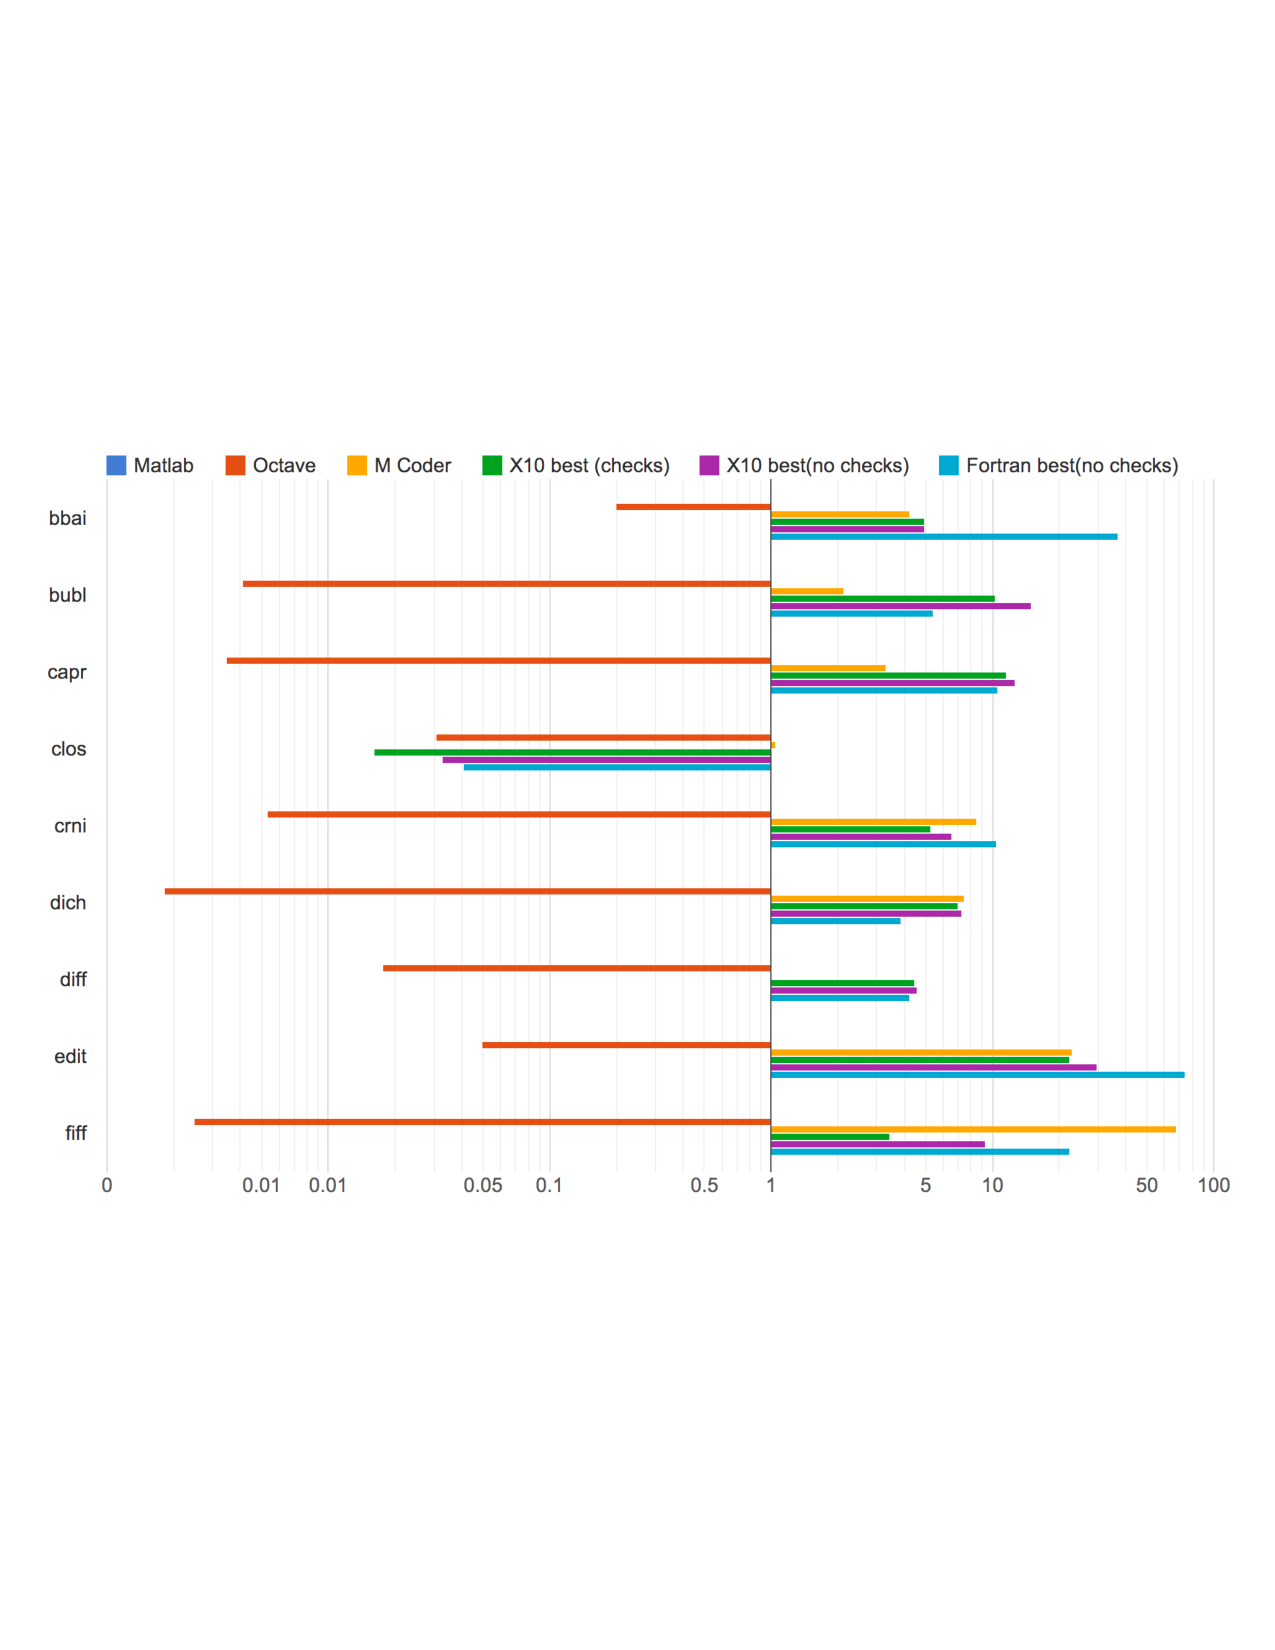
\includegraphics[width=\linewidth]{Figures/final/graph_1_1_1.pdf} \caption
{MiX10 performance comparison (part1) }\label{Fig:graph1_1_1} \end{center}
\end{figure} 
     
\begin{figure}[htbp] \begin{center}
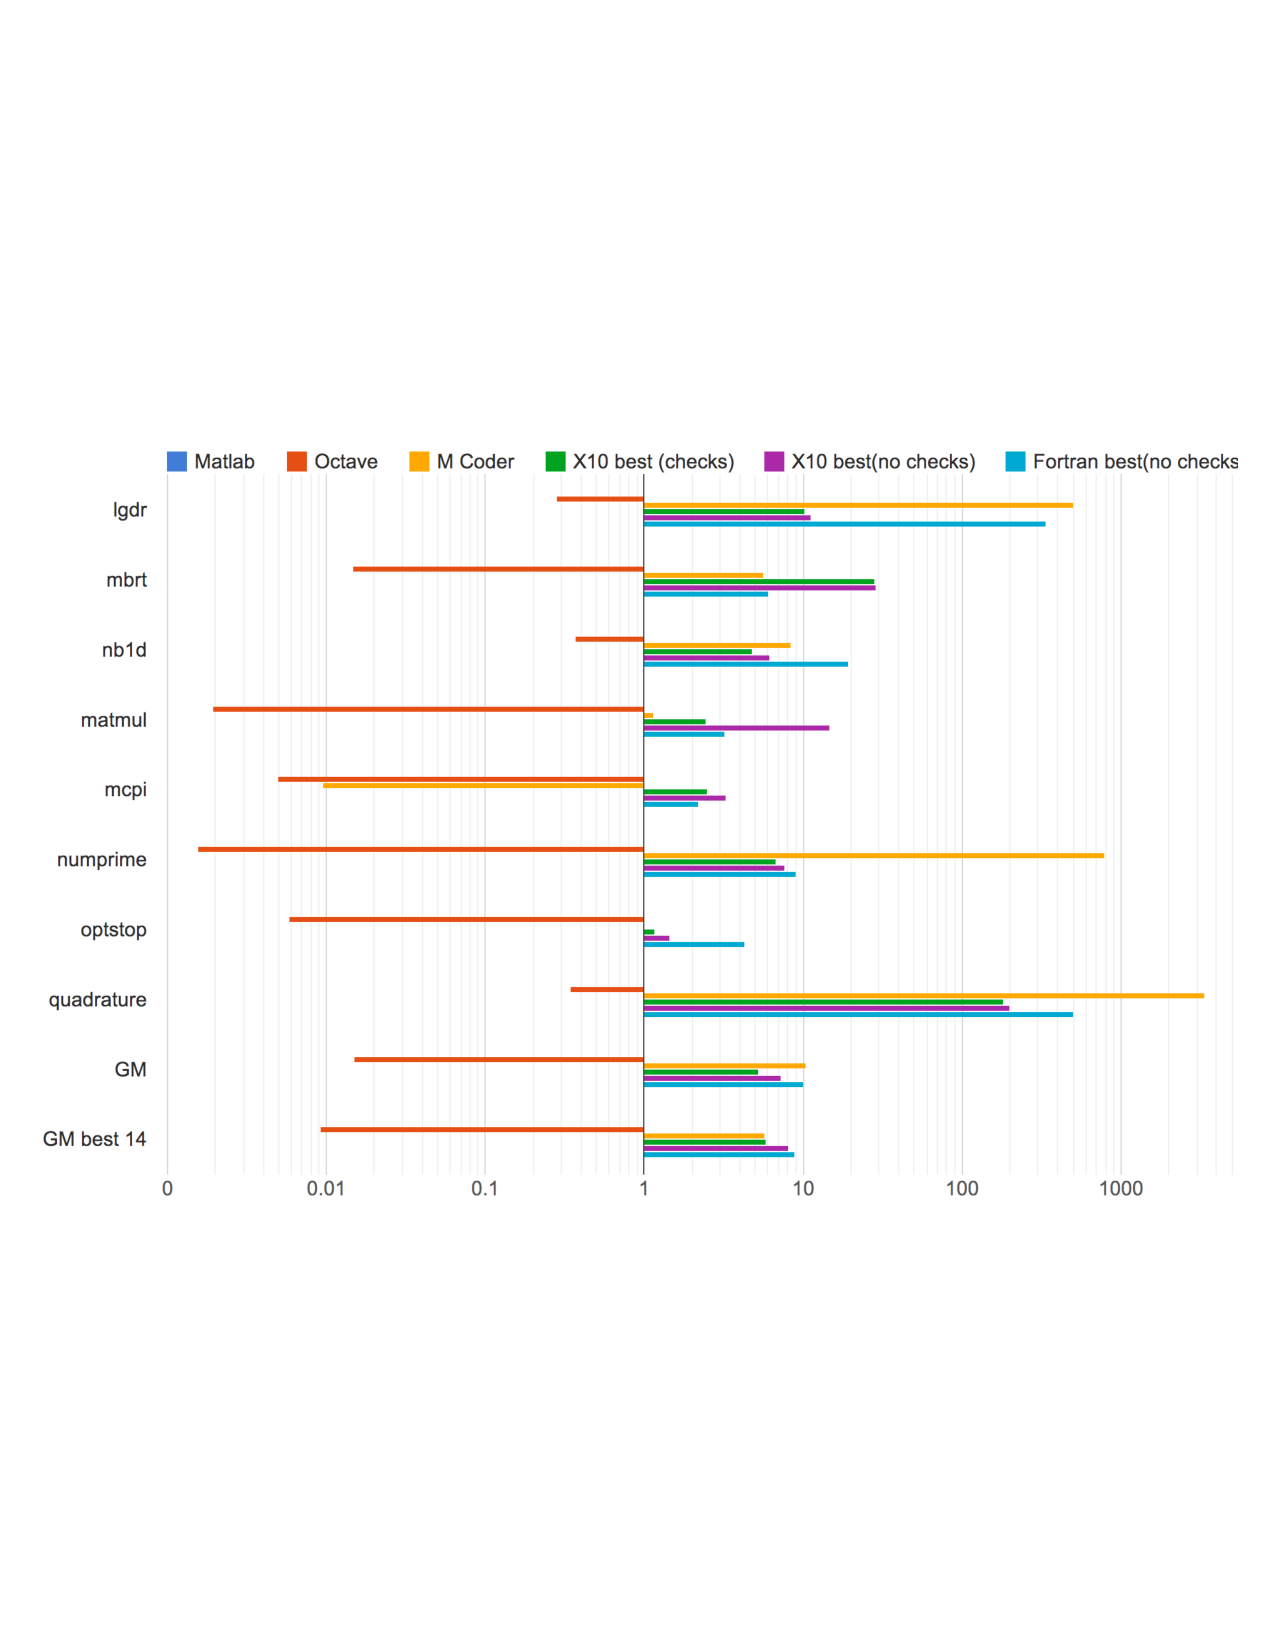
\includegraphics[width=\linewidth]{Figures/final/graph_1_1_2.pdf} \caption
{MiX10 performance comparison (part2) }\label{Fig:graph1_1_2} \end{center}
\end{figure} 

\figref{Fig:graph1_1_1} and \figref{Fig:graph1_1_2} show the speedups and
slowdowns for codes generated for our benchmarks by different compilers.  For
\mixten we have included results for generated \xten code by the \emph{x10c++}
compiler with 1) Array bounds checks turned off; and 2) Array bounds checks
turned on. We used the default optimization provided by the \xten compiler
(\texttt{-O}). For Fortran we included the code generated without bounds checks.
C code from \matlab coder was generated with default settings and includes
bounds checks. \figref{Fig:graph1_1_2} also shows the geometric mean of speedups
for all the benchmarks and for our best 14 out of 17 results (compared to
results from \matlab coder). 

We achieved a mean speedup of 5.2 and 7.2 for x10c++ with bounds checks and
x10c++ with no bounds checks respectively.  On the other hand \matlab coder gave
a mean speedup of 10.5 and \mctwofor gave a mean speedup of 10.2. However, we
see that if we do not consider only three benchmarks for which \xten does not
perform as well as C and Fortran, we get a mean sppedup of 5.75 for x10 with
bounds checks compared to 5.72 for C. For no bounds checks we get a mean speedup
of 8.1 compared to 8.8 for Fortran.  We outperform \matlab coder in 8 out of 17
benchmarks, and Fortran in 7 out of 17 benchmarks

\emph{clos} involves builtin matrix multiplication operations for 2-dimensional
matrices. The generated C code from \matlab coder uses highly optimized matrix
multiplication libraries compared to the naive matrix multiplication
implementation used by \mixten. Thus, we get a speedup of 0.016 as compared to
1.049 for C. Note that the generated Fortran code is also slowed down (speedup
of 0.041) due to the same reason.        

\emph{lgdr} involves repeated transpose of a row vector to a column vector.
\matlab and Fortran, both being array languages are highly optimized for
transpose operations. \mixten currently uses a naive transpose algorithm which
is not as highly optimized. However, we still achieved a speedup of over 10
times. 

\emph{quadrature} solves the stadard quadrature formula for numerical
integration~\cite{}, which involves repeated arithmetic calculations on a range
of numbers. We achieve a speedup of about 200 times compared to \matlab however
it is slow compared to speedups of 3348 and 502 by C and Fortran respectively.
We believe that \matlab coder leverages partial evaluation for optimizing
numerical methods' implementations.

Other interesting numbers are shown by \emph{optstop}, \emph{numprime} and
\emph{fiff}.  \emph{optstop} involves repeated array indexing by an index of
type \texttt{Double} which needs to be explicitly cast to \texttt{Long},
whenever used as an index. IntegerOkay analysis cannot convert it to an integer
type because it's the value returned from a call to the \texttt{floor()}
function whose return type is \texttt{Double}. \emph{numprime} involves similar
problem, where the result of the \texttt{sqrt()} function needs to be converted
to \texttt{Long} from \texttt{Double}. \emph{numprime} also involves a for loop
over a conditional that evaluates to true only once. \matlab coder leverages
this fact for optimizing the for loop by implicitly inserting a \texttt{break}
when the conditional becomes true. We tested our generated \xten code by
explicitly inserting a \texttt{break} statement and achieved a speedup of around
65 times. Note that \emph{numprime} is also used for demonstrating
\texttt{parfor} which does not allow a \texttt{break} statement in the loop.
\emph{fiff} is characterized by stencil operations in a loop, on a 2-dimensional
array. These operations are also optimized by array-based languages like Fortran
and \matlab.  Note that for \emph{nb1d}, Fortran performs better due to the use
of column vectors in the benchmark, which are represented as 2-dimensional
arrays in \xten but in Fortran they are represented as 1-dimensional and are
optimized.

For most of the other benchmarks, we perform better or nearly equal to C and
Fortran code. Inspite of the facts that 1) The sequential core of \xten is a
very high-level object oriented language which is not specialized for
array-based operations; and 2) Generating the executable binaries via \mixten
involves two levels of source-to-source compilations (\matlab $\rightarrow$
\xten $\rightarrow$ C++); We have achieved performance comparable to C and
Fortran.  
       
\section{Comparison of \xten C++ backend and \xten Java backend}

In this section we present the performance comparison for the \mixten generated
\xten code compiled with \xten's C++ backend and that compiled with the \xten's
Java backend. \figref{Fig:graph1_2} shows speedups(slowdowns) for our benchmarks
compiled with 1) \xten C++ backend without bounds checks, 2) \xten C++ backend
with bounds checks, 3) \xten Java backend without bounds checks, and 4) \xten
Java backend with bounds checks. We also show the geometric mean for all our
benchmarks. 

\begin{figure}[htbp] \begin{center}
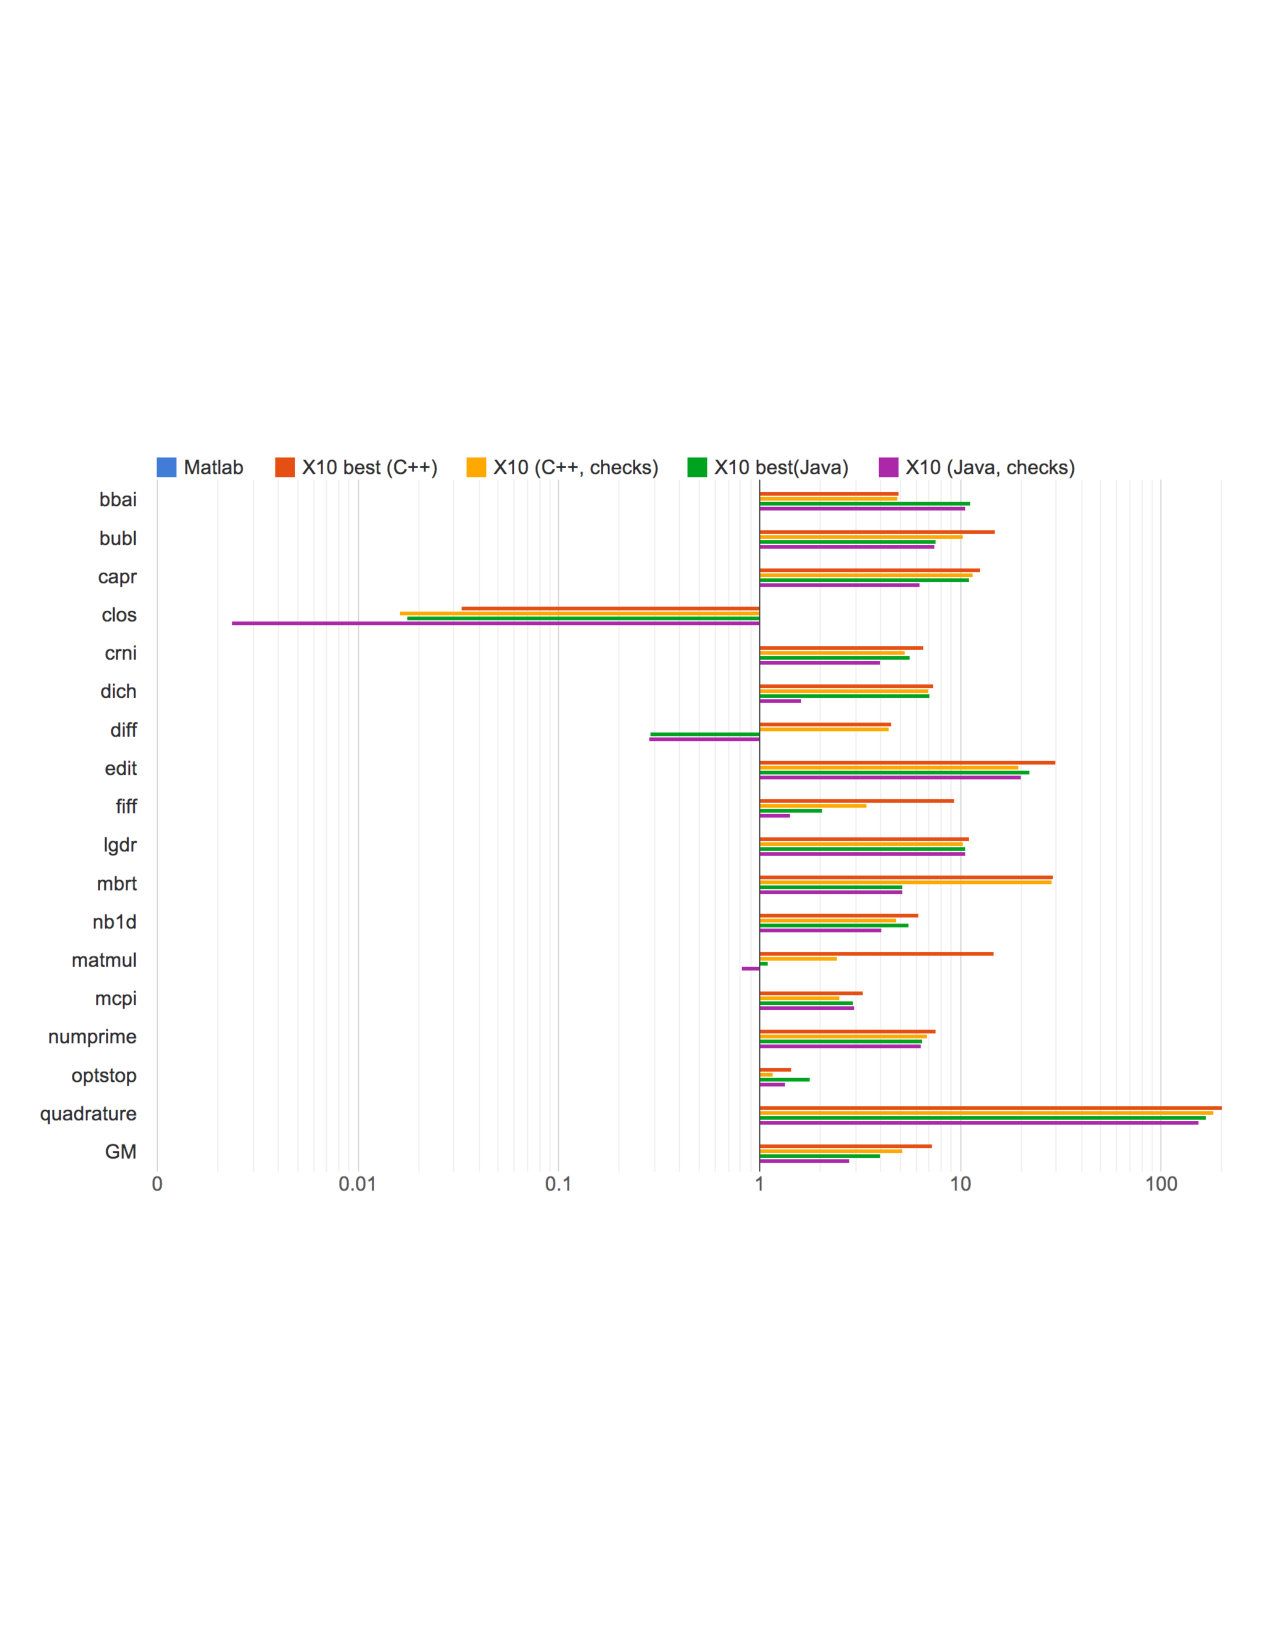
\includegraphics[width=\linewidth]{Figures/final/graph_1_2.pdf} \caption {MiX10
performance comparison : \xten C++ backend vs \xten Java backend}
\label{Fig:graph1_2} \end{center} \end{figure} 

The mean speedups for the C++ backend are 7.22 and 5.16 respectively for bounds
checks switched off, and bounds checks switched on, whereas for Java backend
these values are 3.99 and 2.81 respectively. This is expected, given that C++ is
compiled to native binary while Java is JIT compiled. \emph{bbai} and
\emph{optstop} are the two noticeable exceptions. \emph{bbai} is slow with \xten
C++ backend because it includes repeated calls to the \xten's
\texttt{Random.nextDouble()} function to generate random numbers. We found it to
be significantly slower in the C++ backend compared to the Java backend. We have
reported our findings to the \xten development team and they have validated our
findings. \emph{optstop} is slower for two reasons : \begin{enumerate} \item As
described before, it uses a value of type \texttt{Double} as an array index,
thus requiring a typecast to \texttt{Long}. This is a costly operation since it
involves a check on the value of \texttt{Double} type variable to make sure it
lies within the range of \texttt{Long} type.  \item It also involves random
number generation.  \end{enumerate}  

Other interesting results are for the benchmarks \emph{diff}, \emph{fiff},
\emph{mbrt} and \emph{matmul}. For these benchmarks, results from the Java
backend are significantly slower compared to the C++ backend.  \emph{diff} and
\emph{mbrt} involve operations on complex numbers. In the \xten C++ backend,
complex numbers are stored as \texttt{structs} and are kept on the stack,
whereas in the Java backend, they are stored as \emph{objects} and reside in the
heap storage. \emph{diff} also involves explicit array resizing via \matlab's
concatenation operations which we found to be slower in the Java backend.
\emph{fiff} and \emph{matmul}  are characterized by repeated array access and
read/write operations on 2-dimensional arrays.  For these benchmarks, the Java
backend performs significantly slower compared to the C++ backend with no bounds
checks(2.06 vs. 9.31 for \emph{fiff} and 1.11 vs.  14.72 for \emph{matmul}),
however compared to the performance by the C++ beckend with bounds checks, it is
not as slow(2.06 vs. 3.43 for \emph{fiff} and 1.11 vs.  2.45 for \emph{matmul}).
The reason is that even with bounds checks turned off for the \xten to Java
compiler, The Java compiler by default has bounds checks on. These checks have a
significant effect on performance for 2-dimensional array operations.

\begin{comment} check the large values and enter the exact ones.  \end{comment}

Another important thing to note is that for the benchmarks \emph{capr} and
\emph{dich}, in the case when \xten bounds checks are switched on, we had to
turn off the \xten compiler's optimization switch(\texttt{-O}) to get useful
performance. With the \xten compiler's optimization switch turned on we got a
slowdown of over 2 orders of magnitude.  We recorded running times of 970
seconds for \emph{capr} compared to 3.2 seconds without the optimization, and
1856 seconds for \emph{dich} compared to 12.7 seconds without the optimization.
With the help of the \xten development team we figured out that switching on the
optimization triggered code inlining that caused the resultant Java program to
be too big to be handled by the JIT compiler and reverted to interpretation. 


\section{Comparison of Simple arrays, Region Arrays and specialized Region
arrays}

In this section we discuss the effects on performance due to the use of
different kinds of arrays as described in \chapref{chap:Arrays}.
\figref{Fig:graph2_1} shows the relative speedups and slowdowns for our
benchmarks compiled to use different kinds of \xten arrays for the C++ backend.
\figref{Fig:graph2_2} shows the same results for the Java backend. For this
experiment we considered all the results with \xten compiler optimizations
turned on, and bounds checks turned off.  
   
\begin{figure}[htbp] \begin{center}
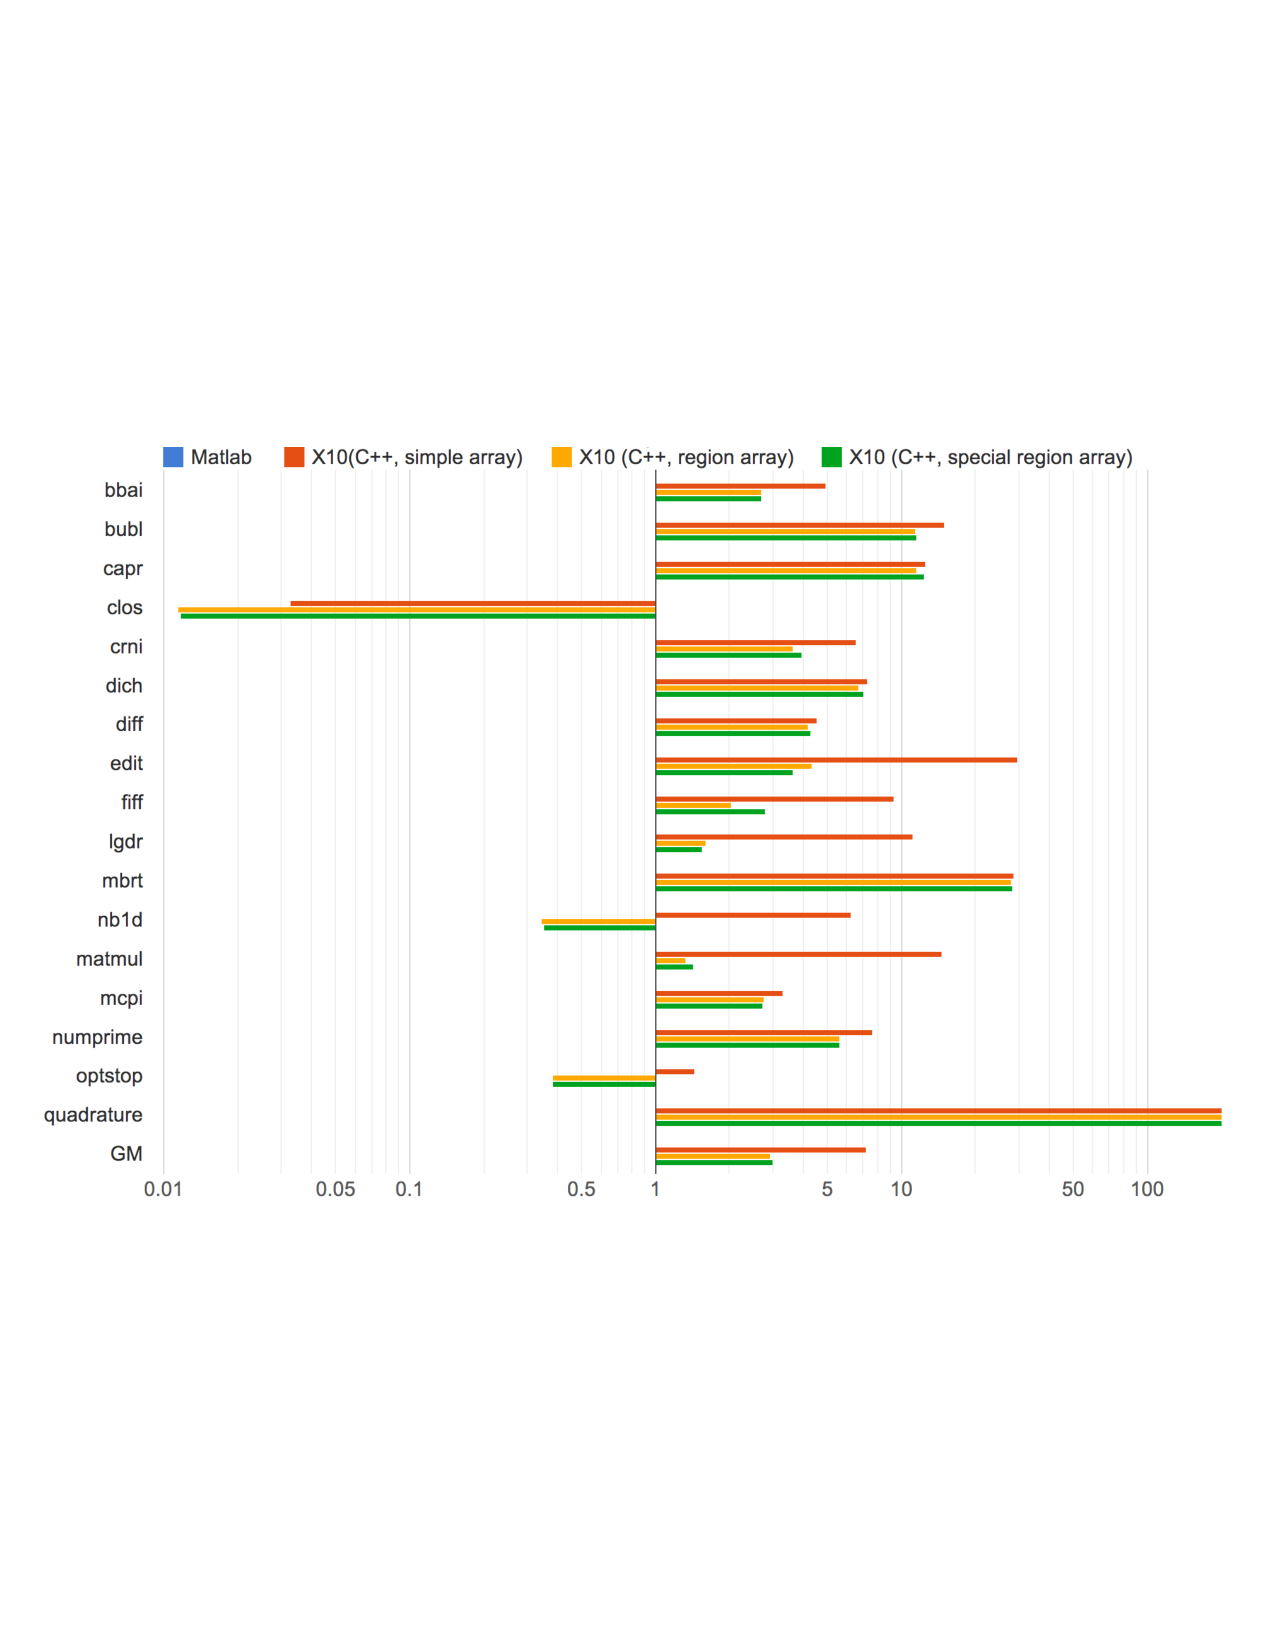
\includegraphics[width=\linewidth]{Figures/final/graph_2_1.pdf} \caption {MiX10
performance comparison : Simple arrays vs. Region arrays vs. specialized Region
Arrays with \xten C++ backend} \label{Fig:graph2_1} \end{center} \end{figure} 

\begin{figure}[htbp] \begin{center}
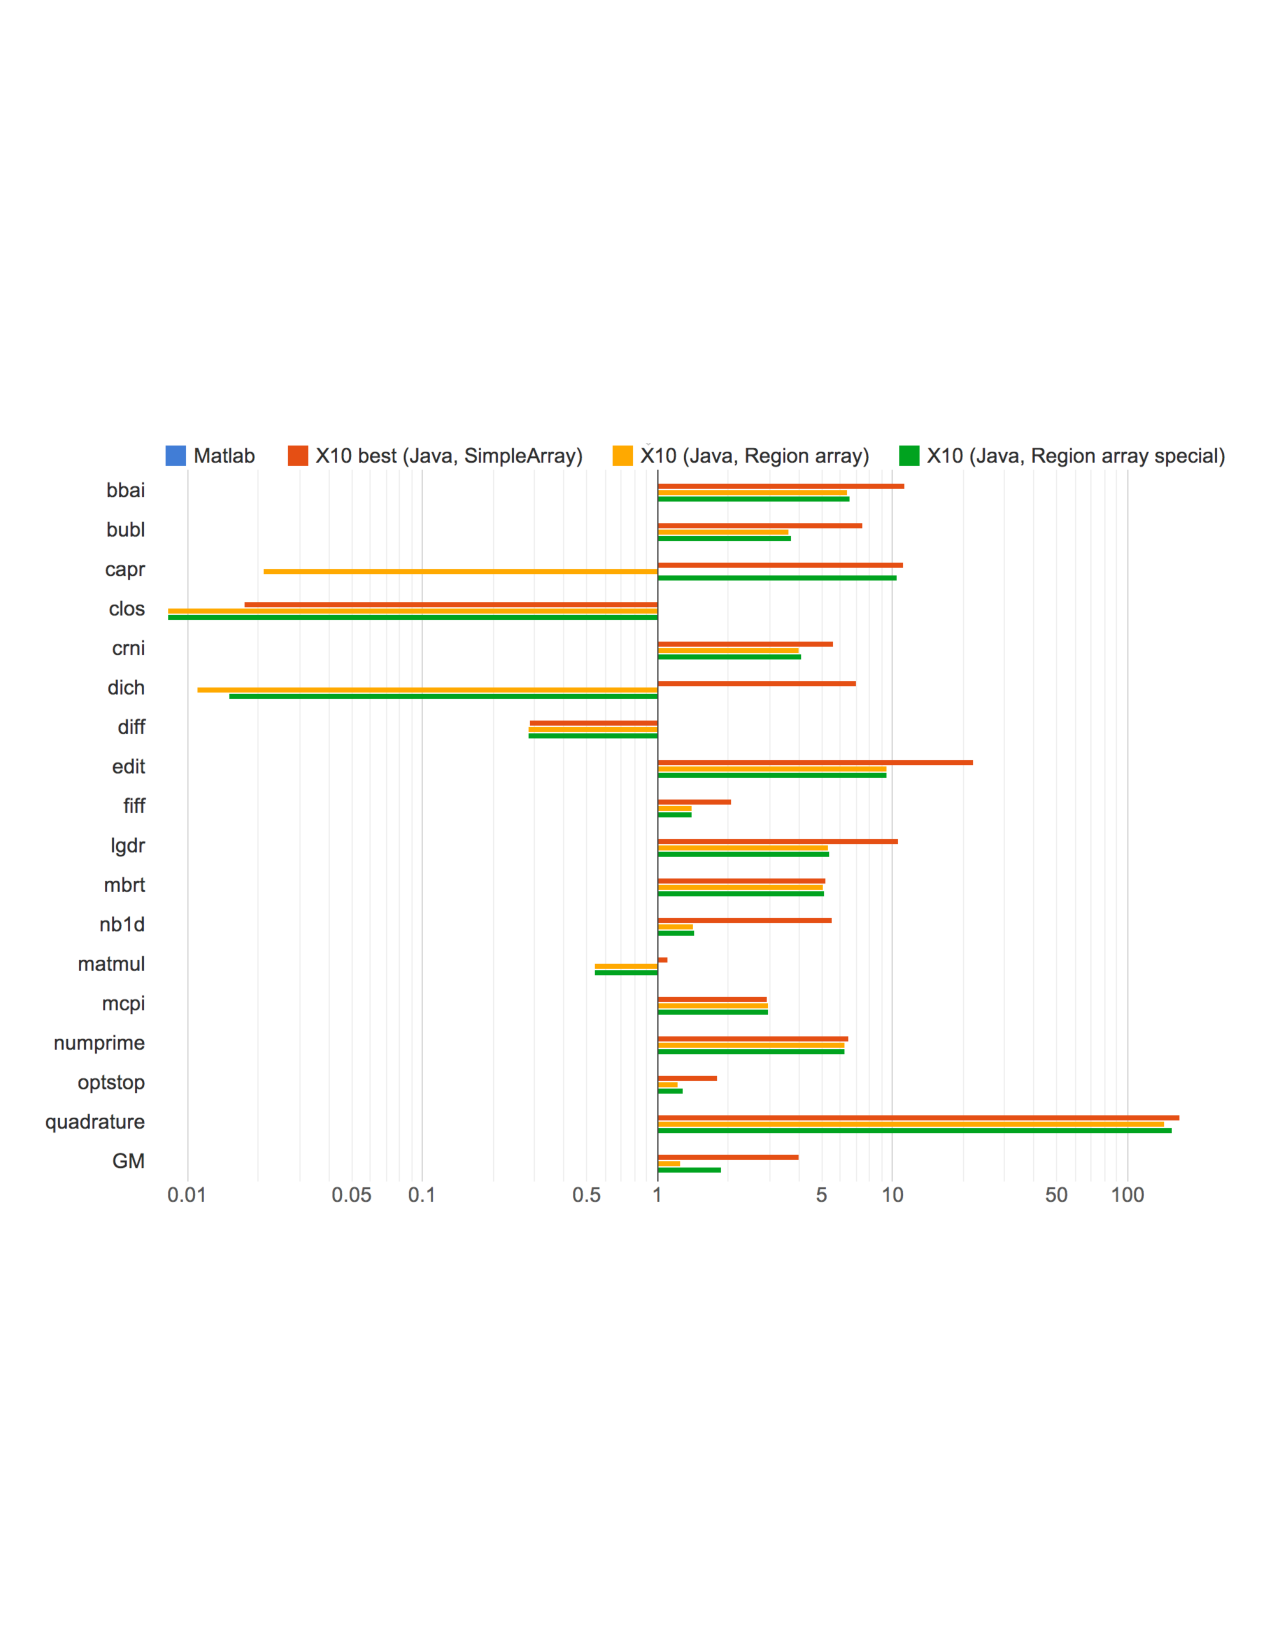
\includegraphics[width=\linewidth]{Figures/final/graph_2_2.pdf} \caption {MiX10
performance comparison : Simple arrays vs. Region arrays vs. specialized Region
Arrays with \xten Java backend} \label{Fig:graph2_2} \end{center} \end{figure}

For the C++ backend we obtained a mean speedup of 7.22 for Simple arrays,
compared to 2.94 for region arrays and 3.02 for specialized region arrays. For
the Java backend, we obtained speedups of 3.99, 1.25 and 1.86 for the simple
arrays, region arrays, and specialized region arrays respectively. These results
are as expected in \chapref{chap:Arrays}. For the C++ backend, most noticeable
performance differences between simple arrays and region arrays are for
\emph{edit}, \emph{fiff}, \emph{lgdr}, \emph{nb1d}, \emph{matmul} and
\emph{optstop}. All of these benchmarks are characterized by large number of
array accesses and read/write operations on 2-dimensional arrays, except
\emph{optstop} and \emph{edit}, which have multiple large 1-dimensional arrays.
Performance difference is most noticeable for \emph{nb1d}, where region arrays
are about 20 times slower than the simple arrays. This is because \emph{nb1d}
involves simple operations on a large column vector. With simple arrays, since
the compiler knows that it is a column vector rather than a 2-dimensional
matrix, even though it is declared as a 2-dimensional array, the performance can
be optimized to match that of the underlying \texttt{Rail}. However, this is not
possible for region arrays where the size of each dimension is not known
statically. For the C++ backend, we do not observe significant performance
differences between region arrays and specialized region arrays.

For the Java backend we obtained higher difference in the mean performance for
the simple arrays and the region arrays. The mean speedup for region arrays is
1.25 whereas for simple arrays it is over 3 times more at 3.99. There is also a
significant difference between the performance of specialized region arrays and
region arrays. Speedup for specialized region arrays is 1.86. Like the C++
backend, here also, most noticeable performance gain for simple arrays id for
benchmarks involving a large number of array accesses and read/writes.
\emph{capr} and \emph{dich} ask for special consideration. For \emph{capr}, even
with \xten compiler's bounds checks turned off, the region array version slows
down by more than 500 times compared to the simple array version and even the
specialized region array version. This again, is due to the fact that region
arrays, with the dynamic shape checks, generated more code than the JIT compiler
could handle. For \emph{dich} the slowdown due to region arrays was about 700
times compared to simple arrays. For \emph{dich}, even the specialization on
region arrays was not enough to reduce the code size enough to be able to be JIT
compiled. 


\section{Performance improvements due to the IntegerOkay analysis}    

In this section we present an overview of the performance improvements achieved
by \mixten by using the IntegerOkay analysis. \figref{fig:graph3_1} and
\figref{fig:graph3_2} show a comparison of speedups gained by using the
IntegerOkay analysis over those without using it. For this experiment we used
results with \xten optimizations turned on and bounds checks turned off. 
   
\begin{figure}[htbp] \begin{center}
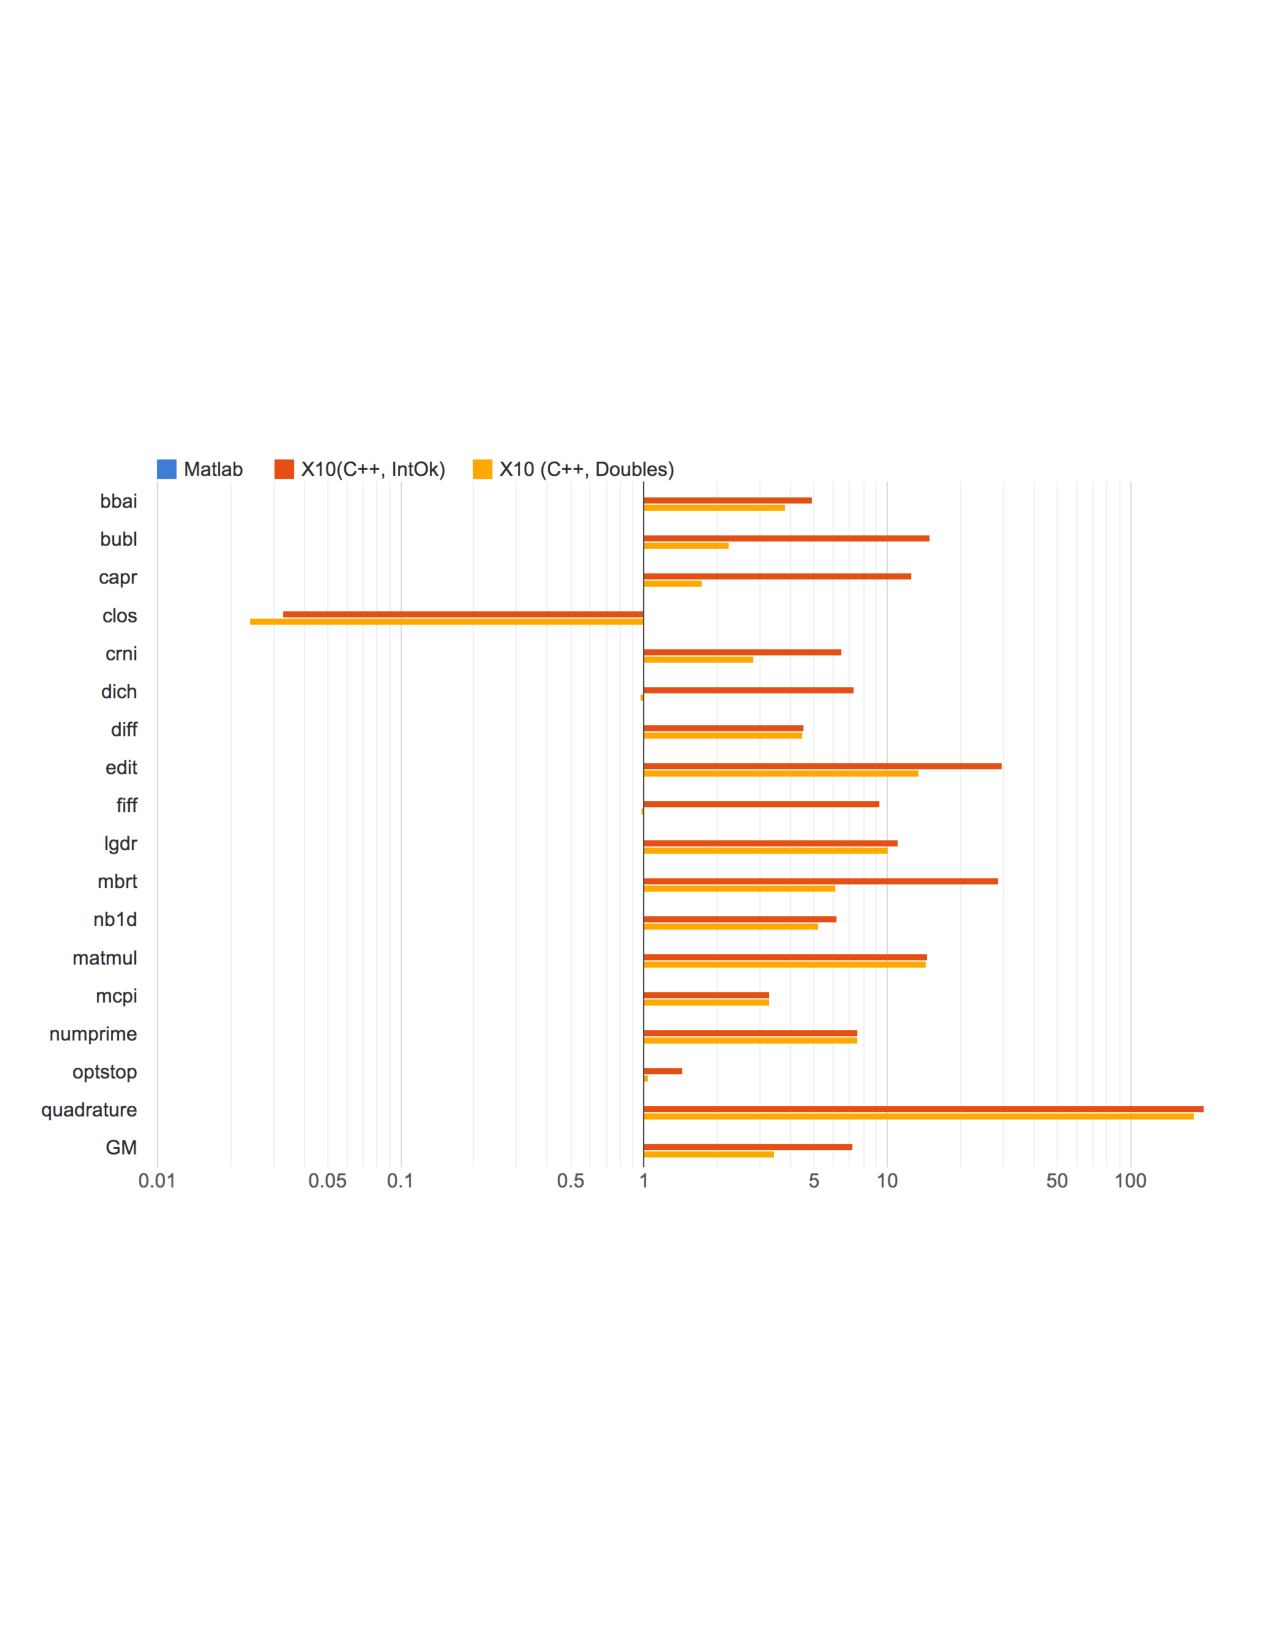
\includegraphics[width=\linewidth]{Figures/final/graph_3_1.pdf} \caption {MiX10
performance comparison : IntegerOkay analysis vs. all \texttt{Double}s with the
\xten C++ backend} \label{Fig:graph3_1} \end{center} \end{figure} 

\begin{figure}[htbp] \begin{center}
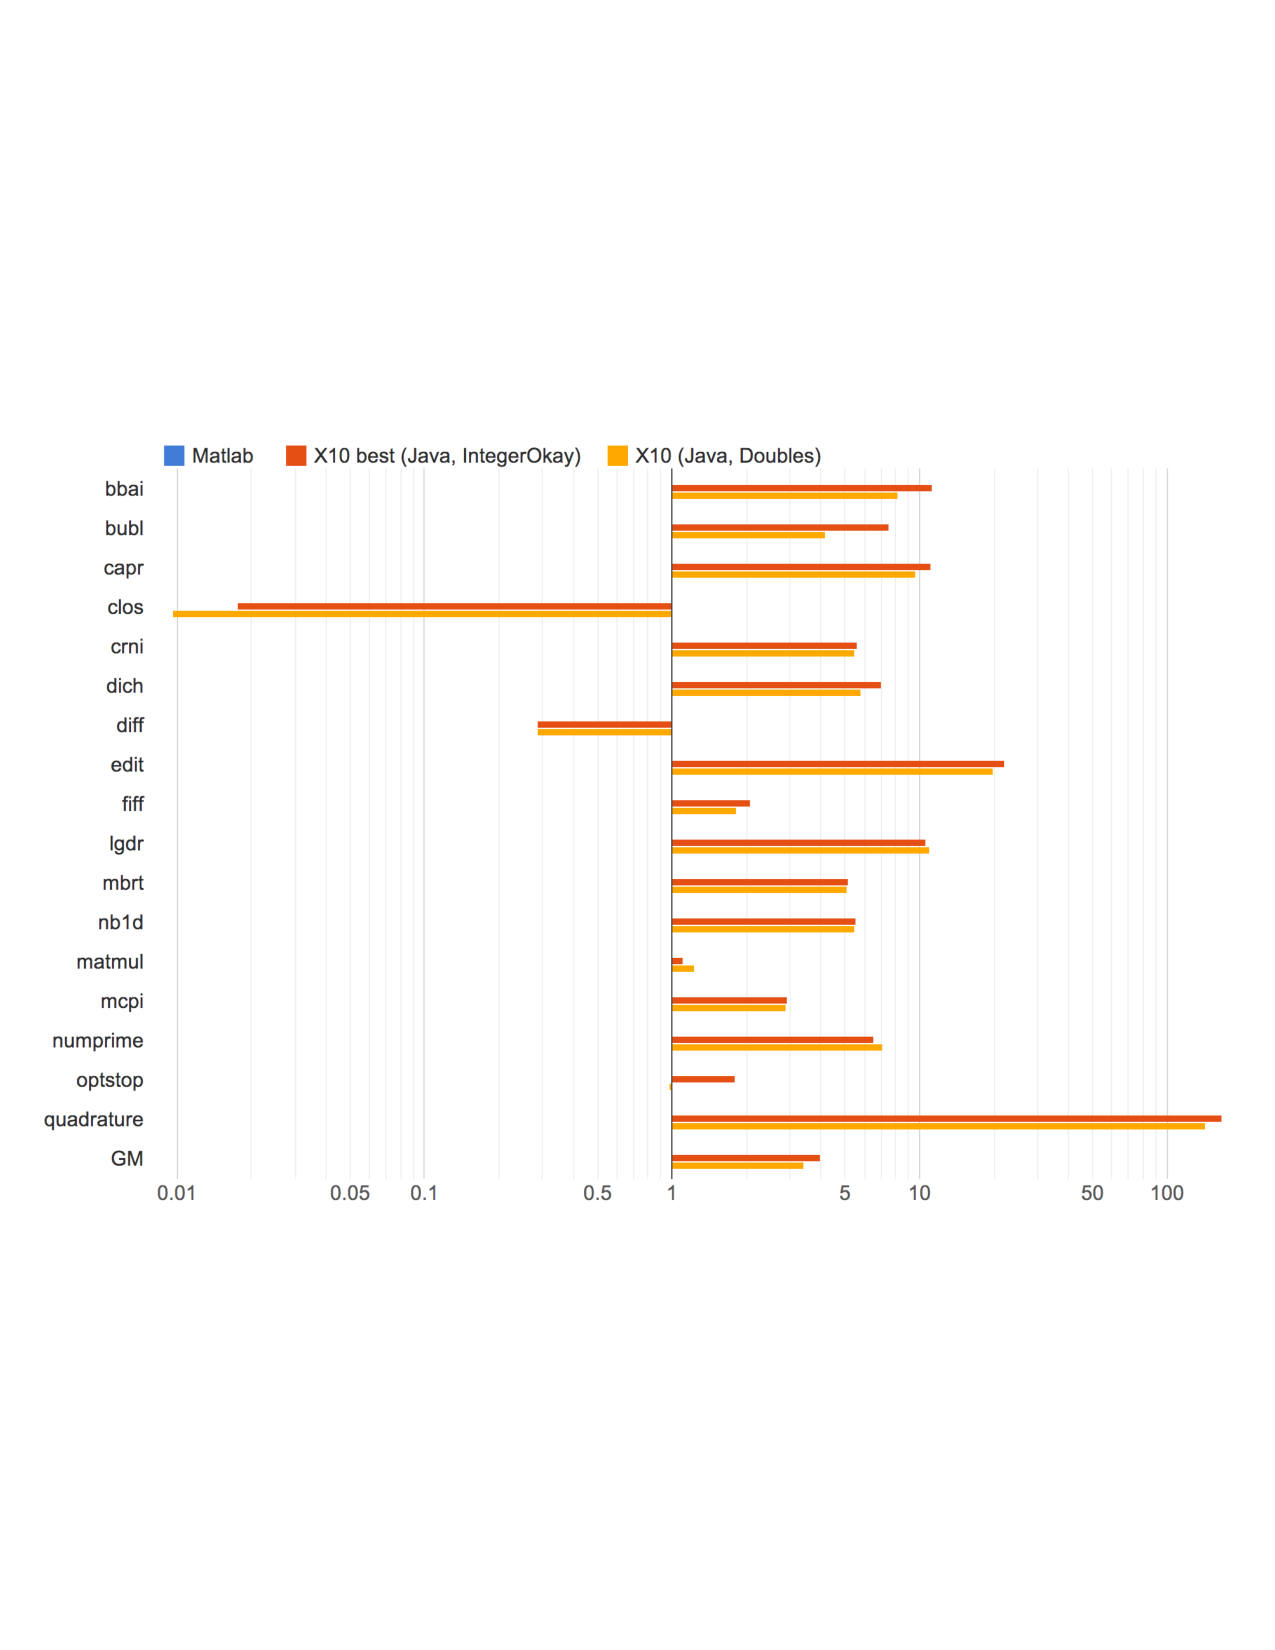
\includegraphics[width=\linewidth]{Figures/final/graph_3_2.pdf} \caption {MiX10
performance comparison : IntegerOkay analysis vs. all \texttt{Double}s with the
\xten Java backend} \label{Fig:graph3_2} \end{center} \end{figure}

For the C++ backend, we observed a mean speedup of 7.22 times which is more than
two times the speedup gained by not using the IntegerOkay analysis, which is
equal to 3.44. We observed a significant gain in performance by using
IntegerOkay analysis for benchmarks that involve significant number of array
indexing operations. \emph{bubl}, \emph{capr}, \emph{crni}, \emph{dich},
\emph{fiff} and \emph{mbrt} show the most significant performance gains. The
reason for this behaviour is that, \xten requires all array indices to be of
type \texttt{Long}, thus if the variables used as array indices are declared to
be of type \texttt{Double} (which is the default in \matlab), they require to be
typecast to \texttt{Long} type. \texttt{Double} to \texttt{Long} is very time
consuming because every cast involves a check on the value of the
\texttt{Double} type variable. 

For the Java backend, with the IntegerOkay analysis, we get a mean speedup of
3.99 as compared to 3.41 without it. The reason for lower difference compared to
that for the C++ backend is that, for Java backend, the \xten compiler does not
generate the value checks for \texttt{Double} type values since these checks are
performed by the JVM which makes them less time consuming. However, we still
notice significant performance difference for the benchmarks which involves
read/write operations on arrays of random numbers. For example, \emph{optstop},
and \emph{bubl} both are nearly twice as fast with the IntegerOkay analysis as
without it. 

To conclude, IntegerOkay analysis is very important for efficient performance of
code involving Arrays, specially for the \xten C++ backend.

\section{performance comparison for \matlab parfor with the \mixten generated
parallel code}

In this section we present the preliminary results for the compilation of
\matlab \texttt{parfor} construct to the parallel \xten code. 7 out of our 17
benchmarks could be safely modified to use the \texttt{parfor} loop.  We compare
the performance of the generated parallel \xten code for these benchmarks to
that of \matlab code using \texttt{parfor} and to their sequential \xten
version. We used the sequential version with optimizations and no bounds checks
and parallel version with optimizations and bounds checks, and with
optimizations and without bounds checks.  \figref{Fig:graph4_1} and
\figref{Fig:graph4_2} show the results for the \xten C++ and the \xten Java
backends respectively.
   
\begin{figure}[htbp] \begin{center}
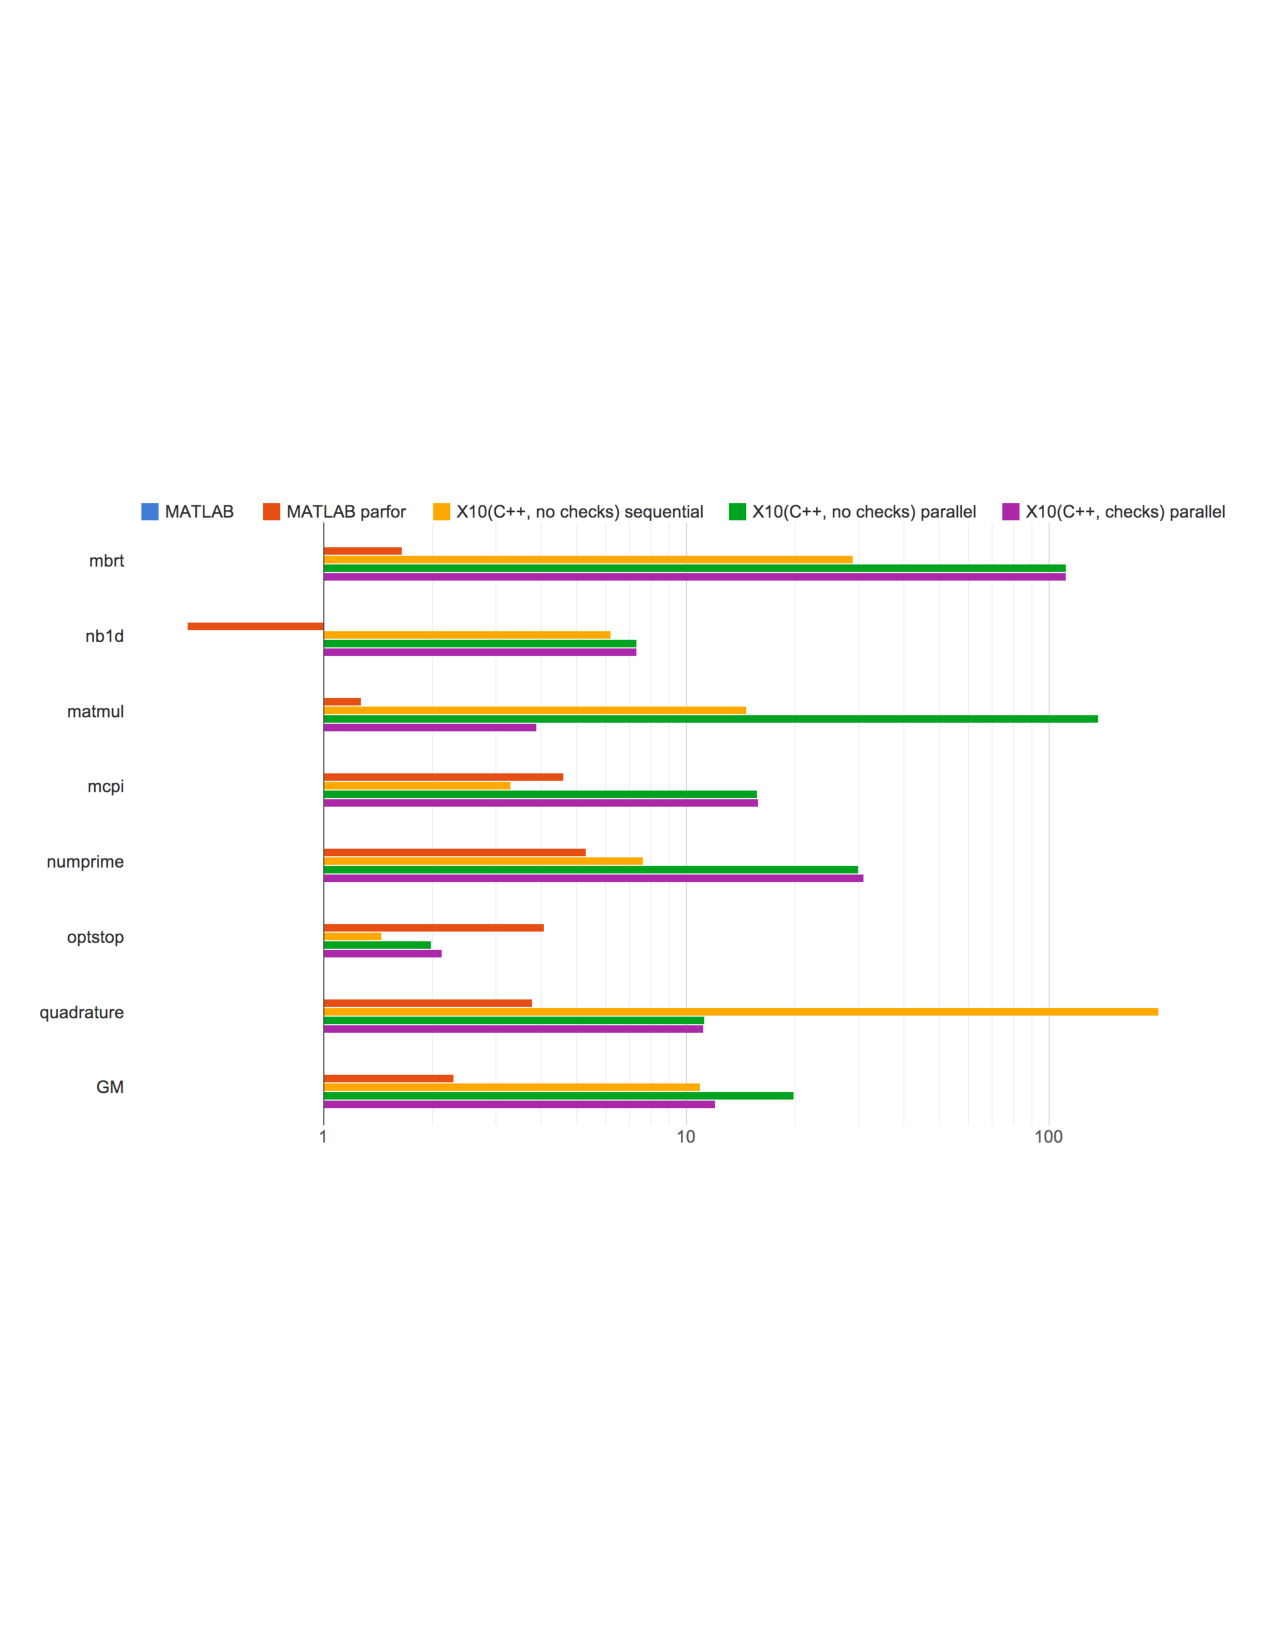
\includegraphics[width=\linewidth]{Figures/final/graph_4_1.pdf} \caption {MiX10
performance comparison : \matlab \texttt{parfor} vs. \mixten generated parallel
\xten code with \xten C++ backend} \label{Fig:graph4_1} \end{center}
\end{figure} 

\begin{figure}[htbp] \begin{center}
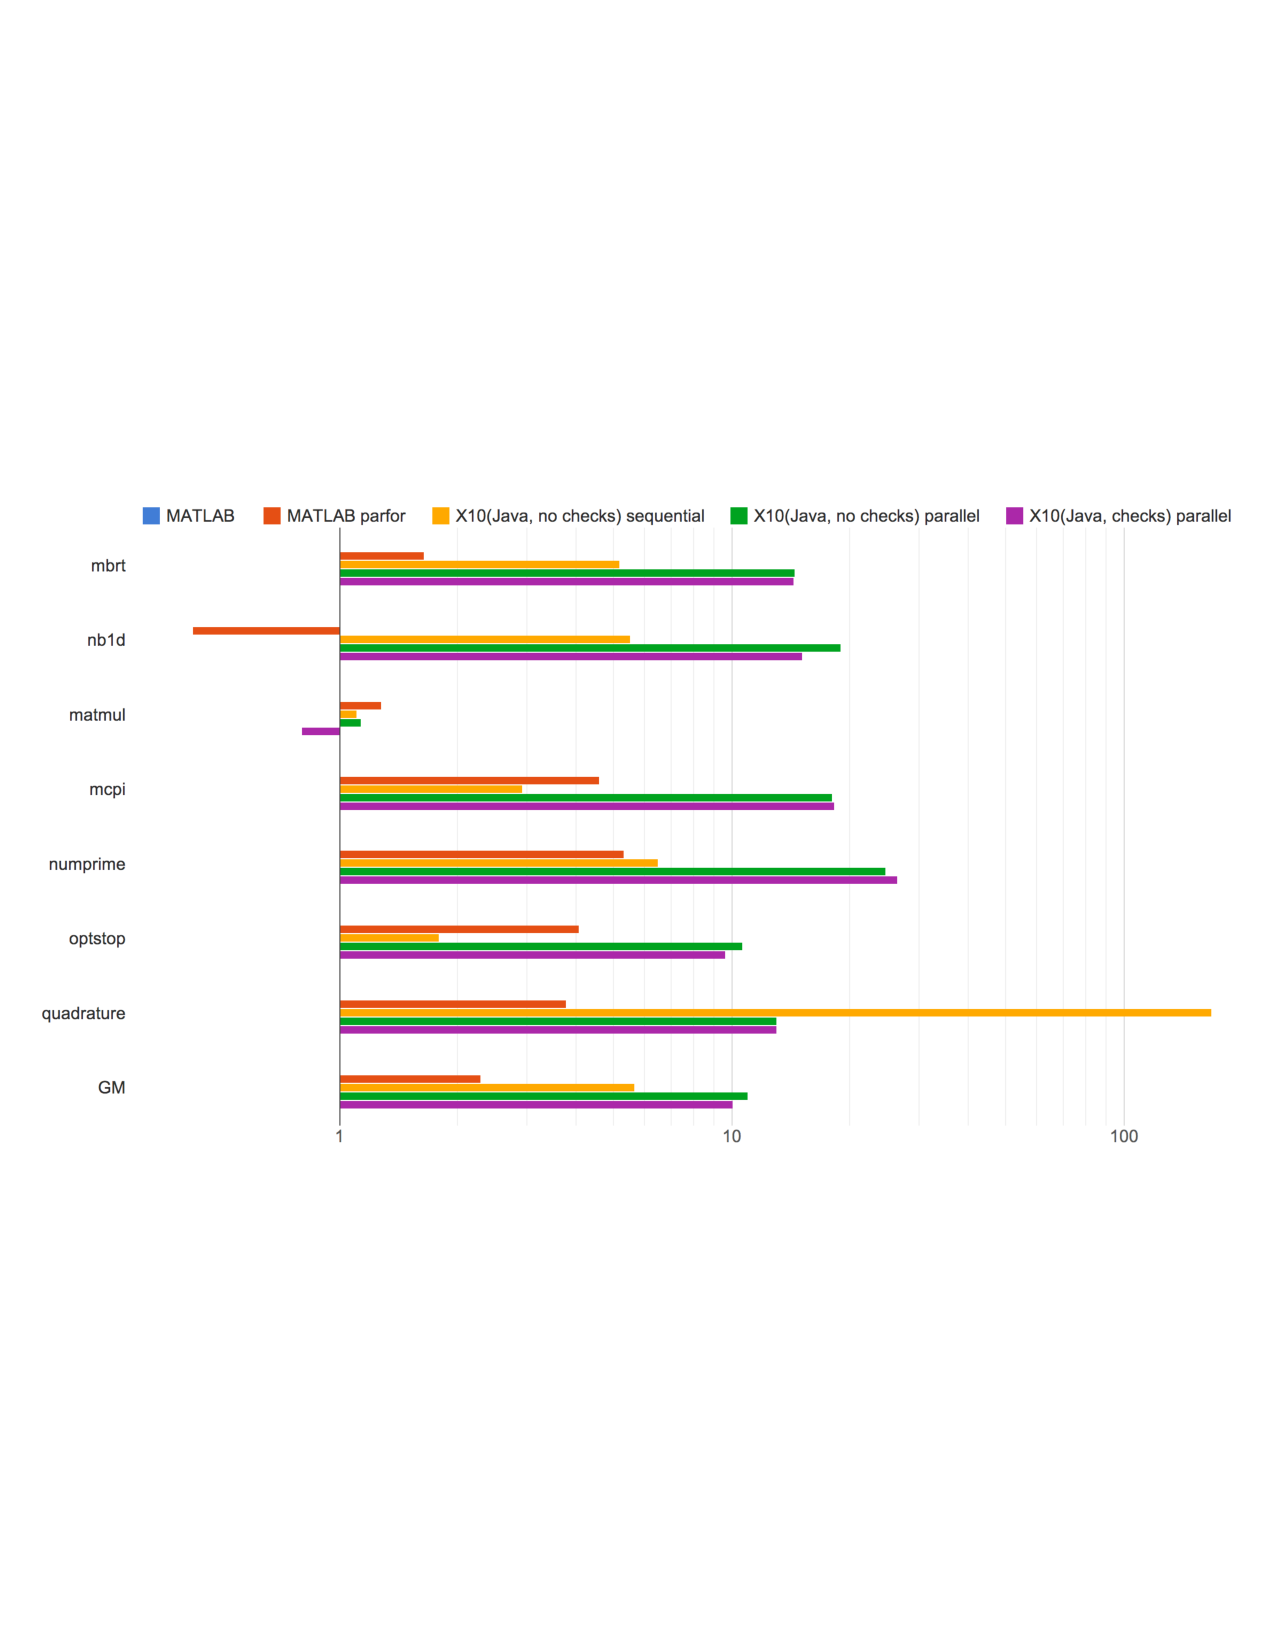
\includegraphics[width=\linewidth]{Figures/final/graph_4_2.pdf} \caption {MiX10
performance comparison : \matlab \texttt{parfor} vs. \mixten generated parallel
\xten code with \xten Java  backend} \label{Fig:graph4_2} \end{center}
\end{figure}

For the \xten C++ backend we achieved a mean speedup of 19.82 for the genereated
parallel \xten code without bounds checks, which is over 9 times of the speedup
for the \matlab code with \texttt{parfor} at a speedup of 2.3. Compared to \xten
sequential code which has a mean speedup of 10.99, it is almost twice as fast.
Even with the parallel \xten code with bounds checks we achieved a speedup of
12.07 which is 5 times better than the \matlab \texttt{parfor} code.
\emph{optstop} is an interesting exception. It is actually slower (at a speedup
of 2.12) than the \matlab \texttt{parfor} version (at a speedup of 4.08). The
sequential version of \emph{optstop} is just slightly faster than the sequential
\matlab version, with a speedup of just 1.45 (due to the reasons explained
earlier) and the total time for the parallel execution of each iteration, and
managing the parallelization of these activities is just slightly faster than
the sequential version. We see a similar trend for the \emph{matmul} benchmark
for the \xten Java backend. It shows a speedup of just 0.8 (version with bounds
checks on) as compared to 1.28 for the \matlab parfor version. Overall, for the
Java backend we obtained a mean speedup of 11.00 for the \xten code with no
bounds checks and 10.09 for the code with bounds checks. Compared to the \matlab
parfor version we obtained over 4 times better performance. The parallel \xten
code is almost 2 times faster than the sequential \xten code (speedup of
5.65).For both, the C++ backend and the Java backend, the mean speedup for the
sequential \xten code is substantially faster than the \matlab parallel code.  

To conclude, the parallel \xten code provides much higher performance gains compared
to the \matlab \texttt{parfor} code  and even the \xten sequential code, which
by itself is most of the times faster than the \matlab parallel code.


\section{Conclusion}

We showed that the \mixten compiler with its efficient handling of array
operations and optimizations like IntegerOkay can generate \xten code that
provides performance comparable to native code generated by languages like C,
which is fairly low-level, and Fortran, which itself is an array-based language.
As a future work, we plan to use more efficient implementations of the builtin
functions, and believe that it would further improve the performance of the code
generated by \mixten.

With \mixten we also took first steps to compile \matlab to parallel \xten code
to take full advantage of the high performance features of \xten. Our
preliminary results are very inspiring and we plan to continue it further in
future.

